
\section*{Problema P11.06}

\renewcommand*\thesection{11.06}
\numberwithin{equation}{section}
\numberwithin{figure}{section}

\begin{center}
    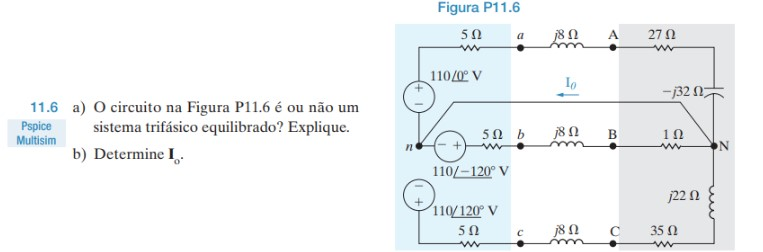
\includegraphics[scale=1.0]{P11.06.jpg}
\end{center}

\subsection*{(a)}

O circuito da Figura P11.6 não é equilibrado pois  
\begin{itemize}
    \item A impedância de cada fase da carga é diferente;
    \item A fonte da fase $c$ não está conectada no neutro da fonte trifásica. Assim, a corrente das fases é diferente e o circuito não é equilibrado.
\end{itemize}

\subsection*{(b)}

Combinando as impedâncias de fase e carga, e usando o fato que a fonte da fase $c$ está desconectada do neutro da fonte trifásica, 
temos o circuito equivalente mostrado na Figura \ref*{fig:11.06.1}.

\begin{figure}[hb]
    \centering
    \caption{Circuito equivalente ao enunciado.}
      \centering
      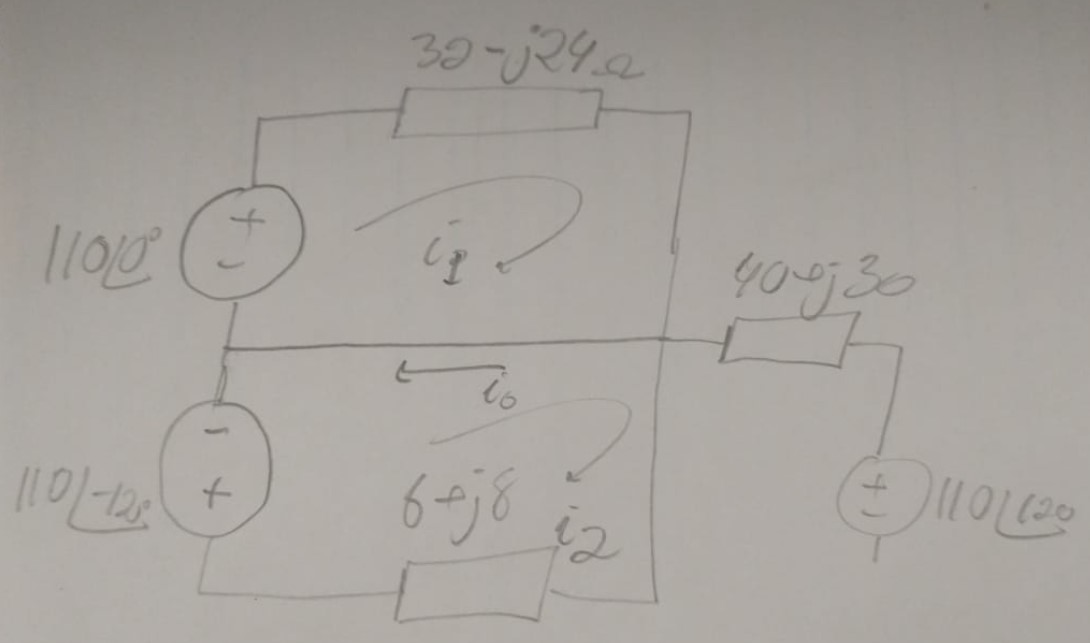
\includegraphics[scale=0.5]{P11.06-Item(b).jpg} \\
    \label{fig:11.06.1}
\end{figure}

Nesse circuito equivalente, aplicamos análise de malhas com as correntes de malha $i_1$ e $i_2$, usando o fato de que   

\begin{equation}\label{eq:11.06.1}
    i_0 = i_1 - i_2
\end{equation}

Malha 1:   

\[ -110 + (32 - j24)i_1 = 0 \]

\[ i_1 = \frac{110}{32 - j24} \]

Malha 2:

\[ 110\fase{-120} + (6 +j8)i_2 = 0 \]

\[ i_2 = - \frac{110\fase{-120}}{6 +j8} \]

Substituindo $i_1$ e $i_2$ em \eqref{eq:11.06.1}, temos   

\[  i_0 =  \frac{110}{32 - j24} - \left(- \frac{110\fase{-120}}{6 +j8}\right)  \]

\[  i_0 =  \frac{110}{32 - j24} - \frac{110\fase{-120}}{6 +j8} \]

\[  i_0 =  2.75\fase{36.86} - 11\fase{-173.13}  \]

\[  i_0 =  2.2 + j1.65 +10.92 + j1.32  \]

\[  i_0 =  13,12 + j2.97 \]

\[ \boxed{i_0 = 13.45\fase{12.75} \un{A}} \]

